%\documentclass[a4paper,10pt]{scrreprt}

\documentclass[12pt,a4paper]{report}
\usepackage{graphicx}

\usepackage[top=2cm,bottom=2cm,left=2cm,right=2cm]{geometry}
\usepackage[utf8]{inputenc}
\usepackage{graphicx}
\usepackage[german]{babel}
\usepackage{pdfpages}
%opening
%\title{ Bloom Filter Implementierung \\ @Diskrete Stochastik}
%\author{Florian Thiévent, Roger Kreienbühl, Stefan Gruber}

\usepackage{fontspec}
\defaultfontfeatures{Mapping=tex-text,Scale=MatchLowercase}
%\setmainfont{TeX}
\setmonofont{Courier New}

\usepackage{fancyhdr}
\renewcommand{\familydefault}{\sfdefault}
\newcommand{\pic}[2][figure]{\begin{figure}[h]
 \centering
 \includegraphics[scale=0.3]{#2}
 % rsc.png: 0x0 pixel, 0dpi, 0.00x0.00 cm, bb=
 \caption{#1}
\end{figure}
}

\usepackage{hyperref}
\hypersetup{
    colorlinks,
    citecolor=black,
    filecolor=black,
    linkcolor=black,
    urlcolor=black
}

\usepackage{framed}
% Code listenings
\usepackage{color}
\usepackage{xcolor}
\usepackage{listings}
\usepackage{caption}
\DeclareCaptionFont{white}{\color{white}}
\DeclareCaptionFormat{listing}{\colorbox{gray}{\parbox{\textwidth}{#1#2#3}}}
\captionsetup[lstlisting]{format=listing,labelfont=white,textfont=white}
\lstset{
 language=Java,
 basicstyle=\footnotesize\ttfamily, % Standardschrift
 numbers=left,               % Ort der Zeilennummern
 numberstyle=\tiny,          % Stil der Zeilennummern
 stepnumber=1,               % Abstand zwischen den Zeilennummern
 numbersep=5pt,              % Abstand der Nummern zum Text
 tabsize=2,                  % Groesse von Tabs
 extendedchars=true,         %
 breaklines=true,            % Zeilen werden Umgebrochen
 frame=b,         
 %commentstyle=\itshape\color{LightLime}, Was isch das? O_o
 %keywordstyle=\bfseries\color{DarkPurple}, und das O_o
 basicstyle=\footnotesize\ttfamily,
 stringstyle=\color[RGB]{42,0,255}\ttfamily, % Farbe der String
 keywordstyle=\color[RGB]{127,0,85}\ttfamily, % Farbe der Keywords
 commentstyle=\color[RGB]{63,127,95}\ttfamily, % Farbe des Kommentars
 showspaces=false,           % Leerzeichen anzeigen ?
 showtabs=false,             % Tabs anzeigen ?
 xleftmargin=17pt,
 framexleftmargin=17pt,
 framexrightmargin=5pt,
 framexbottommargin=4pt,
 showstringspaces=false      % Leerzeichen in Strings anzeigen ?        
}

\begin{document}
\begin{titlepage}
	\centering
	%\includegraphics[width=0.15\textwidth]{example-image-1x1}\par\vspace{1cm}
	\qquad
	\par\vspace{1cm}
	{\scshape\LARGE Fachhochschule Nordwestschweiz \par}
	{\scshape\Large Diskrete Stochastik, HS19\par}
	\vspace{5cm}
	{\huge\bfseries Bloom Filter\par}
	{\scshape\Large Bonusaufgabe\par}
	\vspace{2cm}
	{\Large\itshape  Stefan Gruber \\ Roger Kreienbühl \\ Florian Thiévent \par}
	\vfill
% Bottom of the page
	{\large \today\par}
\end{titlepage}

\tableofcontents
\newpage

\chapter{Idee des BloomFilters}\label{ch:idee-des-bloomfilters}
\section{Vorteile}\label{sec:vorteile}
\section{Nachteile}\label{sec:nachteile}
\begin{lstlisting}
// Hello.java
import javax.swing.JApplet;
import java.awt.Graphics;

public class Hello extends JApplet {
    public void paintComponent(Graphics g) {
        g.drawString("Hello, world!", 65, 95);
    }    
}
\end{lstlisting}

\chapter{Beispiel aus der Praxis}\label{ch:beispiel-aus-der-praxis}
\section{Google Chrome}\label{sec:google-chrome}
Der weitverbreitete Browser Google Chrome benutzt Bloom Filter in seiner Malicious URL Implementierung. Dabei werde URL's die von Usern eingegeben werden durch die Browser Engine geprüft und bei einem positiven Match der User mittels einer Meldung darauf aufmerksam gemacht.

    \begin{figure}[h!]
    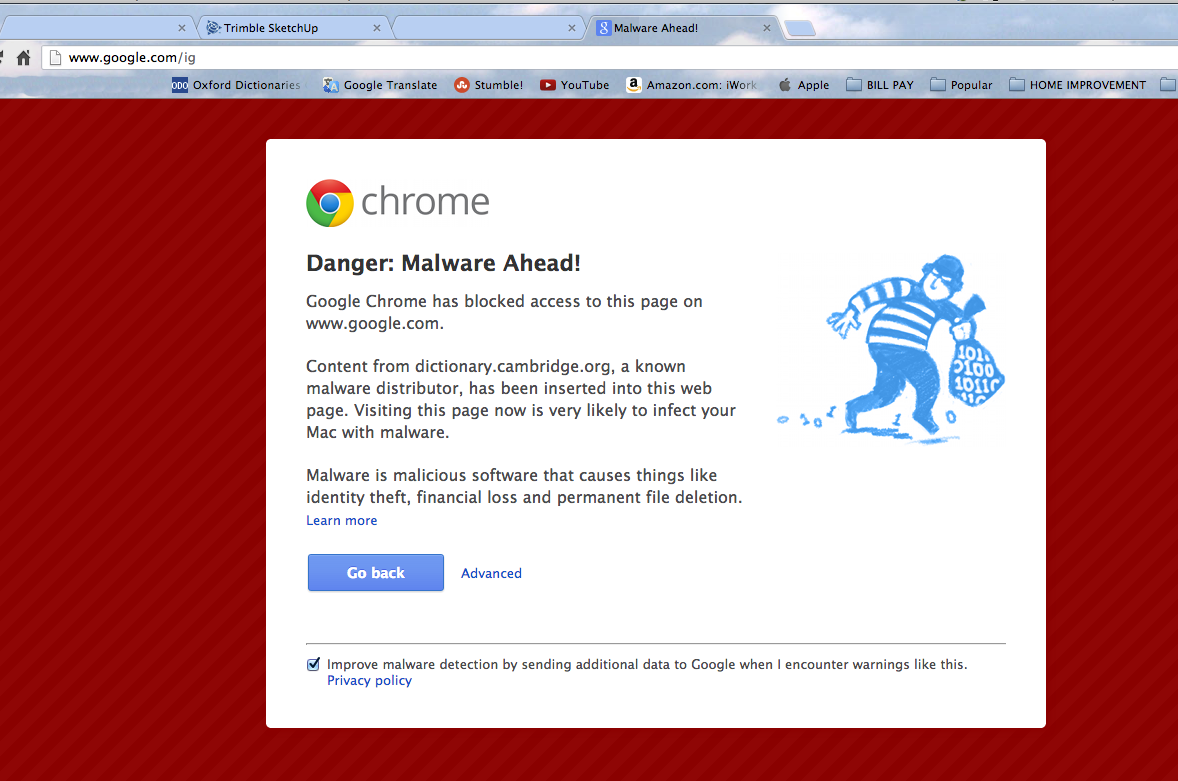
\includegraphics[width=\textwidth]{assets/google_malware.png}
    \caption{Google Chrome Malware Hinweis}
      \label{fig:boat1}
    \end{figure}
    
Die Verwendung eines Bloom Filters bietet sich hier an, das der verwendete Speicherplatz sehr klein ist und die Kommunikation zur Malicious URL API von Google sich damit einen enorm kleinen Footprint hat. Das bedeutet, dass die Abgleiche auch bei einer langsamen Internetverbindung performant durchgeführt werden können.


\chapter{Testergebnisse der Implementierung}\label{ch:testergebnisse-der-implementierung}
\section{Verfahren}\label{sec:verfahren}
\section{Resultate}\label{sec:resultate}
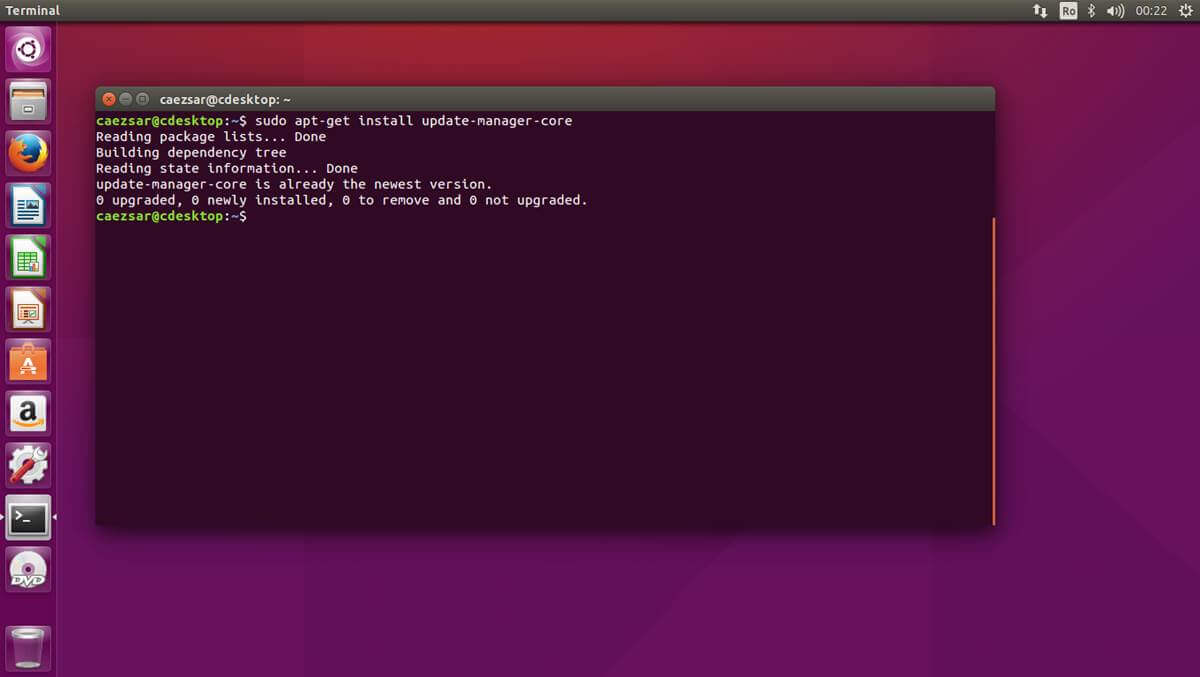
\includegraphics[width=\textwidth]{assets/results.jpg}



\end{document}